\documentclass{article}
\usepackage[utf8]{inputenc}
\usepackage{amsmath, amssymb}
\usepackage{hyperref}
\usepackage{graphicx}
\usepackage{listings}
\usepackage{enumitem}
\usepackage[ruled,vlined]{algorithm2e}
\usepackage{tikz}
\usepackage{multirow}
\usepackage{subfig}
\usepackage[svgnames,table]{xcolor}
\usetikzlibrary{arrows.meta}


\title{Arbitrage Cycle Search Heuristic}
\author{Project Tycho}
\date{\today}

\newcommand{\xin}{x_{\text{in}}}
\newcommand{\yout}{y_{\text{out}}}

\usetikzlibrary{shadows, arrows.meta,decorations.markings,positioning,calc,fit}
\tikzset{
  tokenstyle/.style={
    rectangle,
    rounded corners,
    draw=black,
    fill=white,
    drop shadow,
    font=\scriptsize,
  }
}

\begin{document}

\maketitle

\tableofcontents

\section{Overview}
The Tycho Searcher processes real-time blockchain data and identifies arbitrage opportunities. It receives block updates from a data feed, maintains an up-to-date graph of token exchanges, and applies a modified Bellman-Ford algorithm to detect negative cycles, which correspond to profitable arbitrage paths.

\section{System Architecture}
\begin{itemize}[leftmargin=*, label=--]
    \item \textbf{Tycho Feed:} An asynchronous task receives block updates and token data from an external source, and forwards them to the searcher.
    \item \textbf{Searcher:} The searcher maintains the exchange graph, updates it with new data, and runs the arbitrage detection algorithm.
 \end{itemize}
The code is written in rust. It uses asynchronous channels (\texttt{tokio::sync::mpsc}) to communicate between the feed and the searcher.


\section{Searcher Workflow}
\begin{enumerate}[leftmargin=*, label=\arabic*.]
    \item \textbf{Initialization:} The searcher initializes its graph structures and awaits block updates.
    \item \textbf{Block Update Handling:} Upon receiving a new block, the searcher updates the graph with the latest exchange rates and liquidity data.
    \item \textbf{Arbitrage Detection:} The searcher runs the modified Bellman-Ford algorithm to find negative cycles, which indicate arbitrage opportunities.
    \item \textbf{Result Export:} The searcher processes the detected opportunities and can export or log them for further action.
\end{enumerate}

\section{Modified Bellman-Ford Algorithm}
\subsection{Purpose}
The Bellman-Ford algorithm can detect negative cycles in a weighted graph. We have adapted the algorithm to search arbitrage cycles, in order to find cycles with positive profit in the exchange graph. We also consider that the internal state of an Automated Market Maker (AMM) changes after each exchange. We therefore restrict arbitrage cycles to traverse each AMM no more than once.

\subsection{Data Structures}
\begin{itemize}[leftmargin=*, label=--]
    \item \texttt{Graph}: This is a directed graph. Each node represents a token. And each edge corresponds to an AMM and represents the exchange rates between the corresponding tokens.
    \item \texttt{Edge Weights}: 
Each edge $e$ is associated with two functions: $w_e(\xin)$ and $g_e(\xin)$. Here, $w_e(\xin)$ returns the amount of tokens received after the swap, $\yout$. Meanwhile, $g_e(\xin)$ returns the gas used. This is typically a constant function, because the gas cost is usually independent of $\xin$.
\end{itemize}

We assume that $w_e(\xin)$ is a monotone non-decreasing function; that is, increasing the input amount $\xin$ does not decrease the output amount $\yout$. Moreover, the exchange rate $\frac{\yout}{\xin}$ is a monotone non-increasing function of $\xin$.

Each query to $e()$ incurs a computational cost. In practice, a Rust call implements this to \texttt{get\_amount\_out}, which emulates the swap. Both $\xin$ and $\yout$ are stored as large integer values.


\begin{figure}
\centering
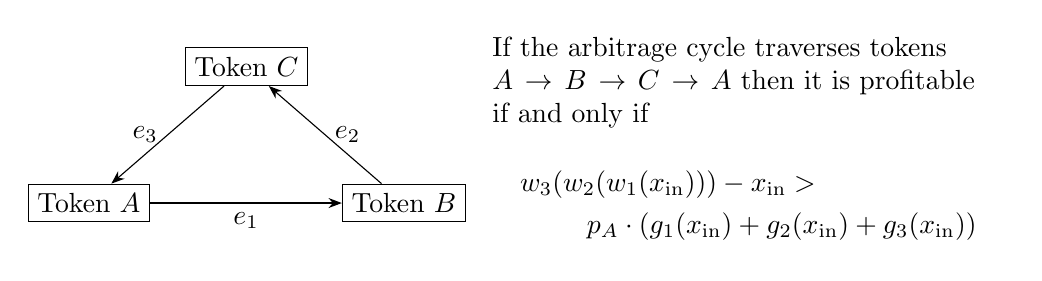
\begin{tikzpicture}[>=Stealth, node distance=2cm]
\node[draw] (A) at (0,0) {Token $A$};
\node[draw] (B) at (4,0) {Token $B$};
\node[draw] (C) at (2,1.732) {Token $C$}; % Equilateral triangle
\draw[->] (A) -- node[below] {$e_1$} (B);
\draw[->] (B) -- node[right] {$e_2$} (C);
\draw[->] (C) -- node[left] {$e_3$} (A);
\node[anchor=west, text width=65mm, align=left] at (5,0.8) {If the arbitrage cycle traverses tokens $A \rightarrow B \rightarrow C \rightarrow A$ then it is profitable if and only if 
\begin{multline*}
w_3(w_2(w_1(\xin))) - \xin > \\ p_A\cdot (g_1(\xin) + g_2(\xin) + g_3(\xin))
\end{multline*}
};
\end{tikzpicture}
\caption{An illustration of arbitrage cycle. $p_A$ is the exchange rate for Token $A$ in ether.}\label{fig:arbcycle}
\end{figure}

Fig.~\ref{fig:arbcycle} illustrates an example of an arbitrage cycle. An arbitrage is defined by a closed path in the (exchange) graph and an input amount $\xin$, which is denominated in the start token. The cycle begins and ends at the same token, which we refer to as the \emph{start node} or \emph{start token}.

Arbitrage cycles have two key performance metrics:
\begin{enumerate}
\item Gas cost: the sum of the gas used by each pool along the arbitrage path, including inter-pool transfers;
\item Profit: the net gain in the amount of the start token.
\end{enumerate}

Gas is paid in Ether. So determining whether an arbitrage is profitable requires knowing the start token's price $p$ in ETH. If the start token is WETH, then $p = 1$.

It is important to note that the function $e()$ changes after each swap. Fig. \ref{fig:arbcycle} thus only holds if the three edges belong to different AMMs. For each edge, we therefore explicitly store the pool to which it belongs.

\begin{itemize}[leftmargin=*, label=--]
    \item \texttt{Pools}:  For each edge $e$ we store the associated pool $p(e)$. 
\end{itemize}
    
We restrict the search space to cycles in which every edge belongs to a different pool; that is, for any cycle $C$ and any distinct edges $e,f \in C$, we require $p(e)\neq p(f)$. Although some studies do not impose this restriction on the problem space \cite{diamandis2024convex}, we find that in practice, it has only a minimal impact on solution quality.

\subsection{Precomupations}

As a first step, we decompose the graph into 2-edge-connected components. This enables us to search within each cycle independently.
A 2-edge-connected component is a maximal set of nodes in which every pair of nodes is connected by at least two edge-disjoint paths. For any two nodes in the component, an equivalent cycle passes through each node – even if the cycle is not simple (e.g., it may consist of a figure-eight shape).
This subdivision has several advantages: upon an update, only the affected components need to be recomputed; and the search is also easily parallelizable (although we have not implemented parallelization in our prototype).

In practice, we apply a slightly stronger decomposition, because we know the starting token (node) of the arbitrage cycles (e.g., WETH) in advance.
As a first step, we consider the 2-edge-connected component of the graph that contains the start node. Tokens that are either unreachable from the start node through AMMs, or reachable only via a single AMM, are irrelevant for the purpose of cycle detection.
Next, we temporarily remove the starting node (e.g., WETH) from the graph and compute the connected components of the remaining graph.
When we re-add the starting node, each of these components becomes a subgraph that is only connected to the rest of the graph through the starting node.
This effectively “splits” the search space into independent parts.
It is easy to see that we can search cycles independently in these subgraphs, because any cycle that would traverse multiple components can only cross via the starting node. Any hypothetical cycle that spans multiple components must pass through the starting node. And such a cycle can always be decomposed into smaller cycles contained entirely within individual subgraphs.

\begin{figure}
\centering
\tikzset{
    token/.style={circle, draw, thick, minimum size=7mm, inner sep=0pt, font=\small, fill=white},
    start/.style={draw=black, fill=yellow!30, very thick},
    faint/.style={token, draw=gray!70, fill=gray!10, text=gray!70},
    unreachable/.style={token, draw=gray!60, fill=gray!15},
    amm/.style={<->, thick},
    weak/.style={<->, dashed, gray!70},
    compbox/.style={draw, rounded corners, inner sep=3pt, thick},
    label/.style={font=\footnotesize, align=center}
 }
\subfloat[Original graph with start node WETH]{
\begin{tikzpicture}[]
% Start node
\node[start] (S) at (0,2) {\strut WETH};
% Cluster left (C1-ish around WETH)
\node[token] (a1) at (-1.5,3.2) {A1};
\node[token] (a2) at (-2.3,2.0) {A2};
\node[token] (a3) at (-1.5,0.8) {A3};
\node[token] (a4) at (-0.4,3.1) {A4};
% Edges around S (multiple AMMs)
\draw[amm] (S) -- (a1);
\draw[amm] (S) -- (a3);
\draw[amm] (S) -- (a4);
% Internal edges in left cluster (to hint at 2-edge-connectivity)
\draw[amm] (a1) -- (a2);
\draw[amm] (a2) -- (a3);
\draw[amm] (a3) -- (a1);
\draw[amm] (a1) -- (a4);
% Right cluster (C2)
\node[token] (b1) at (2.0,3.0) {B1};
\node[token] (b2) at (3.0,2.0) {B2};
\node[token] (b3) at (2.0,1.0) {B3};
%
\draw[amm] (S) -- (b2);
\draw[amm] (b1) -- (b2);
\draw[amm] (b2) -- (b3);
\draw[amm] (b3) -- (b1);
% A token reachable only via a single AMM from S (faint)
\node[faint] (x1) at (0.2,0.2) {X};
\draw[weak] (S) -- (x1);
% Unreachable component (grey, no link to S)
\node[unreachable] (u1) at (-3.5,2.8) {U1};
\node[unreachable] (u2) at (-4.2,1.8) {U2};
\node[unreachable] (u3) at (-3.6,0.8) {U3};
\draw[weak] (u1) -- (u2);
\draw[weak] (u2) -- (u3);
\draw[weak] (u3) -- (u1);
\node[label, anchor=north] at (-3.8,0.3) {\scriptsize Unreachable from WETH};
\end{tikzpicture}}
\\
\subfloat[Step1: Remove start node. Identify the connected components of $G \setminus \{\text{WETH}\}$]{\qquad
\begin{tikzpicture}[]
% (No start node here)
% Left component C1
\node[token] (a1b) at (-1.5,3.2) {A1};
\node[token] (a2b) at (-2.3,2.0) {A2};
\node[token] (a3b) at (-1.5,0.8) {A3};
\node[token] (a4b) at (-0.4,3.1) {A4};
\draw[amm] (a1b) -- (a2b);
\draw[amm] (a2b) -- (a3b);
\draw[amm] (a3b) -- (a1b);
\draw[amm] (a1b) -- (a4b);
\node[compbox, fit=(a1b)(a2b)(a3b)(a4b), label] (C1box) {};
\node[label, above=1pt of C1box.north] {\scriptsize $C_1$};
% Right component C2
\node[token] (b1b) at (2.0,3.0) {B1};
\node[token] (b2b) at (3.0,2.0) {B2};
\node[token] (b3b) at (2.0,1.0) {B3};
\draw[amm] (b1b) -- (b2b);
\draw[amm] (b2b) -- (b3b);
\draw[amm] (b3b) -- (b1b);
\node[compbox, fit=(b1b)(b2b)(b3b), label] (C2box) {};
\node[label, above=1pt of C2box.north] {\scriptsize $C_2$};
% Single-edge node becomes singleton (could be filtered out)
\node[faint] (x1b) at (0.2,0.2) {X};
\node[compbox, draw=gray!60, fit=(x1b)] (C3box) {};
\node[label, below=1pt of C3box.south] {\scriptsize $C_3$ (singleton)};
% Unreachable stays its own component
\node[unreachable] (u1b) at (-3.5,2.8) {U1};
\node[unreachable] (u2b) at (-4.2,1.8) {U2};
\node[unreachable] (u3b) at (-3.6,0.8) {U3};
\draw[weak] (u1b) -- (u2b);
\draw[weak] (u2b) -- (u3b);
\draw[weak] (u3b) -- (u1b);
\node[compbox, draw=gray!60, fit=(u1b)(u2b)(u3b)] (C0box) {};
\node[label, above=1pt of C0box.north] {\scriptsize $C_0$ (unreachable)};
\end{tikzpicture}\qquad\qquad}
\\
\subfloat[Add start node back. Independent subgraphs via WETH]{
\begin{tikzpicture}[]
% Start node again
\node[start] (Sc) at (0,2) {\strut WETH};
% C1 + WETH subgraph
\node[token] (a1c) at (-1.5,3.2) {A1};
\node[token] (a2c) at (-2.3,2.0) {A2};
\node[token] (a3c) at (-1.5,0.8) {A3};
\node[token] (a4c) at (-0.4,3.1) {A4};
\draw[amm] (Sc) -- (a1c);
\draw[amm] (Sc) -- (a3c);
\draw[amm] (Sc) -- (a4c);
\draw[amm] (a1c) -- (a2c);
\draw[amm] (a2c) -- (a3c);
\draw[amm] (a3c) -- (a1c);
\node[compbox, fit=(a1c)(a2c)(a3c)(a4c)(Sc)] (S1) {};
\node[label, above=1pt of S1.north,xshift=-1cm] {\scriptsize Subgraph $S_1 = C_1 \cup \{\text{WETH}\}$};
% C2 + WETH subgraph
\node[token] (b1c) at (2.0,3.0) {B1};
\node[token] (b2c) at (3.0,2.0) {B2};
\node[token] (b3c) at (2.0,1.0) {B3};
\draw[amm] (Sc) -- (b2c);
\draw[amm] (b1c) -- (b2c);
\draw[amm] (b2c) -- (b3c);
\draw[amm] (b3c) -- (b1c);
\node[compbox, fit=(b1c)(b2c)(b3c)(Sc)] (S2) {};
\node[label, above=1pt of S2.north,xshift=2cm] {\scriptsize Subgraph $S_2 = C_2 \cup \{\text{WETH}\}$};
% Singleton / filtered (optional)
\node[faint] (x1c) at (0.2,0.2) {X};
\draw[weak] (Sc) -- (x1c);
\node[label] at (0.3,-0.4) {\scriptsize (single-edge, often ignored)};
\end{tikzpicture}}
\caption{Decompose the graph into components for arbitrage cycle search}
\end{figure}

Table \ref{table:graph} reports the graph size, the number of connected components, and the size of the largest component, as a function of the set of pools under consideration. The pools include Uniswap v2, v3, and v4, Ekubo v2, Balancer v2, and Curve. We further filter pools by their total value locked (TVL), measured in Ether.
The table shows that this step yields a significant speedup. For instance, in a graph with $2\,375$ nodes, the largest component contains only $367$ nodes. This illustrates how special the structure of the graph is.

See also Fig. \ref{fig:token_graph}, which shows the graph skeleton of the largest component. This is a simplified representation produced by first removing self-loops and iteratively pruning leaves (degree‑1 nodes), then collapsing degree‑2 chains into single edges marked as skeleton (and marking these edges as dashed lines). These transformations preserve the graph for a cycle search.


\begin{table}
\caption{Performance of the algorithm for pools of various minimum TVL values. }
\label{table:graph}
\centering
\small
\begin{tabular}{cr|rr|r|rr|r}
\hline
\multicolumn{2}{c|}{AMMs} &  \multicolumn{2}{c|}{full graph}& \#compo-& \multicolumn{2}{c|}{largest component} & runtime\\
types&TVL &\#nodes&\#edges&nents&\#nodes&\#edges& \\
\hline
\multirow{3}{*}{\rotatebox{90}{\footnotesize
  \parbox{1.2cm}{\centering Uniswap v2,3,4 Ekubo Balancer curve}}}
&1000 & 111 & 322 & 54 & 47 & 190 & 4.2 s \\
&100 & 623 & 1662 & 435 & 166 & 574 & 12 s \\
&10 & 2467 & 6164 & 1980 & 462 &1924 & 21 s \\
\hline
\multirow{3}{*}{\rotatebox{90}{\footnotesize
  \parbox{1.2cm}{\centering Uniswap v2, v3}}}
&1000 & 78 & 202 & 42 & 26 & 90 & 40 ms \\
&100 & 563 & 1324 & 420 & 126 & 398 & 271 ms \\
&10 & 2375 & 5470 & 1973 & 367 & 1258 & 359 ms \\
\end{tabular}
\end{table}

\begin{figure}
\definecolor{prot_uniswap_v2}{HTML}{FF0000}  % protocol: uniswap_v2
\definecolor{prot_uniswap_v3}{HTML}{0000FF}  % protocol: uniswap_v3
\definecolor{prot_uniswap_v4}{HTML}{00AA00}  % protocol: uniswap_v4
\definecolor{prot_balancer_v2}{HTML}{FF7700}  % protocol: vm:balancer_v2
\definecolor{prot_curve}{HTML}{9900CC}  % protocol: vm:curve
\subfloat[All pools]{
%!TEX root = ../searcher_documentation.tex
\begin{tikzpicture}[>=stealth, yscale=0.7, xscale=0.8]
  \node[tokenstyle] (deUSD) at (-2.969cm, 4.798cm) {deUSD};
  \node[tokenstyle] (ZARP) at (-2.904cm, 2.710cm) {ZARP};
  \node[tokenstyle] (ANGLE) at (-7.550cm, 0.931cm) {ANGLE};
  \node[tokenstyle] (CRV) at (1.505cm, -0.463cm) {CRV};
  \node[tokenstyle] (ICHI) at (0.810cm, -3.282cm) {ICHI};
  \node[tokenstyle] (DAI) at (-1.775cm, -1.305cm) {DAI};
  \node[tokenstyle] (DOLA) at (1.011cm, 4.645cm) {DOLA};
  \node[tokenstyle] (frxETH) at (6.912cm, 1.556cm) {frxETH};
  \node[tokenstyle] (ELON) at (-4.817cm, -0.777cm) {ELON};
  \node[tokenstyle] (cbBTC) at (1.347cm, 1.549cm) {cbBTC};
  \node[tokenstyle] (msETH) at (8.250cm, 0.792cm) {msETH};
  \node[tokenstyle] (HEZ) at (-6.162cm, -2.094cm) {HEZ};
  \node[tokenstyle] (WETH) at (0.006cm, -0.908cm) {WETH};
  \node[tokenstyle] (USDf) at (-5.606cm, 3.957cm) {USDf};
  \node[tokenstyle] (TONCOIN) at (-1.552cm, 2.825cm) {TONCOIN};
  \node[tokenstyle] (USDC) at (-1.234cm, 0.317cm) {USDC};
  \node[tokenstyle] (PYUSD) at (-1.779cm, 4.319cm) {PYUSD};
  \node[tokenstyle] (LINK) at (1.644cm, 0.321cm) {LINK};
  \node[tokenstyle] (USDT) at (-2.521cm, 0.846cm) {USDT};
  \node[tokenstyle] (PAXG) at (-4.304cm, 0.160cm) {PAXG};
  \node[tokenstyle] (FOOM) at (2.262cm, -3.288cm) {FOOM};
  \node[tokenstyle] (PEPE) at (3.451cm, -3.077cm) {PEPE};
  \node[tokenstyle] (INV) at (2.863cm, 3.140cm) {INV};
  \node[tokenstyle] (HEX) at (-3.618cm, -0.826cm) {HEX};
  \node[tokenstyle] (wstETH) at (5.000cm, 0.106cm) {wstETH};
  \node[tokenstyle] (XYO) at (-5.868cm, -1.214cm) {XYO};
  \node[tokenstyle] (UNI) at (1.980cm, -2.009cm) {UNI};
  \node[tokenstyle] (EURC) at (-4.308cm, 2.369cm) {EURC};
  \node[tokenstyle] (ENA) at (-2.902cm, -4.142cm) {ENA};
  \node[tokenstyle] (USDe) at (-0.504cm, 1.776cm) {USDe};
  \node[tokenstyle] (DOLO) at (-7.750cm, 2.284cm) {DOLO};
  \node[tokenstyle] (wQUIL) at (-6.449cm, -0.328cm) {wQUIL};
  \node[tokenstyle] (Mog) at (-2.441cm, -6.070cm) {Mog};
  \node[tokenstyle] (AAVE) at (4.013cm, -0.839cm) {AAVE};
  \node[tokenstyle] (SOTU) at (2.322cm, -5.462cm) {SOTU};
  \node[tokenstyle] (RLB) at (-5.896cm, 0.574cm) {RLB};
  \node[tokenstyle] (OUSD) at (2.413cm, 3.968cm) {OUSD};
  \node[tokenstyle] (FET) at (-1.707cm, -4.254cm) {FET};
  \node[tokenstyle] (SHIB) at (3.900cm, -5.217cm) {SHIB};
  \node[tokenstyle] (EURA) at (-6.832cm, 2.967cm) {EURA};
  \node[tokenstyle] (ODIN) at (-0.543cm, -3.824cm) {ODIN};
  \node[tokenstyle] (rust) at (0.842cm, -4.333cm) {rust};
  \node[tokenstyle] (crvUSD) at (1.158cm, 2.314cm) {crvUSD};
  \node[tokenstyle] (XAUt) at (-3.963cm, -1.935cm) {XAUt};
  \node[tokenstyle] (OLAS) at (-1.299cm, -2.819cm) {OLAS};
  \node[tokenstyle] (SKY) at (-5.626cm, -3.179cm) {SKY};
  \node[tokenstyle] (GHO) at (-0.254cm, 3.826cm) {GHO};
  \node[tokenstyle] (OHM) at (2.852cm, -1.030cm) {OHM};
  \node[tokenstyle] (SPX) at (6.769cm, -3.547cm) {SPX};
  \node[tokenstyle] (USD1) at (-5.338cm, 2.146cm) {USD1};
  \node[tokenstyle] (APU) at (5.154cm, -4.706cm) {APU};
  \node[tokenstyle] (HUNT) at (-4.757cm, 1.288cm) {HUNT};
  \node[tokenstyle] (1INCH) at (4.450cm, -1.937cm) {1INCH};
  \node[tokenstyle] (WBTC) at (0.857cm, -1.687cm) {WBTC};
  \node[tokenstyle] (FRAX) at (2.529cm, 1.418cm) {FRAX};
  \node[tokenstyle] (PEAS) at (-1.366cm, -5.347cm) {PEAS};
  \node[tokenstyle] (USR) at (-0.375cm, 5.930cm) {USR};
  \node[tokenstyle] (tBTC) at (3.338cm, 0.670cm) {tBTC};
  \node[tokenstyle] (OETH) at (6.385cm, 2.753cm) {OETH};
  \node[tokenstyle] (CVX) at (4.278cm, 1.461cm) {CVX};
  \node[tokenstyle] (USDS) at (-4.038cm, -3.594cm) {USDS};
  \node[tokenstyle] (BITCOIN) at (5.791cm, -1.574cm) {BITCOIN};
  \node[tokenstyle] (ENS) at (-2.578cm, -2.491cm) {ENS};
  \draw[draw=prot_curve, solid] (deUSD) -- (DOLA);
  \draw[draw=prot_curve, solid] (deUSD) -- (USDC);
  \draw[draw=prot_curve, solid] (deUSD) -- (USDT);
  \draw[draw=prot_uniswap_v3, solid] (ZARP) -- (USDC);
  \draw[draw=prot_uniswap_v3, solid] (ZARP) -- (WETH);
  \draw[draw=prot_uniswap_v3, solid] (ZARP) -- (USDT);
  \draw[draw=prot_uniswap_v3, solid] (ANGLE) -- (WETH);
  \draw[draw=prot_uniswap_v4, solid] (ANGLE) -- (USDT);
  \draw[draw=prot_uniswap_v3, dashed] (ANGLE) -- (EURA);
  \draw[draw=prot_uniswap_v2, solid] (CRV) -- (UNI);
  \draw[draw=prot_uniswap_v3, solid] (CRV) -- (WETH);
  \draw[draw=prot_uniswap_v4, solid] (CRV) -- (CVX);
  \draw[draw=prot_uniswap_v3, solid] (CRV) -- (USDT);
  \draw[draw=prot_uniswap_v3, solid] (CRV) -- (USDC);
  \draw[draw=prot_uniswap_v4, solid] (CRV) -- (rust);
  \draw[draw=prot_curve, solid] (CRV) -- (crvUSD);
  \draw[draw=prot_uniswap_v3, solid] (ICHI) -- (WBTC);
  \draw[draw=prot_uniswap_v3, solid] (ICHI) -- (USDC);
  \draw[draw=prot_uniswap_v2, dashed] (ICHI) -- (WETH);
  \draw[draw=prot_uniswap_v4, solid] (DAI) -- (USDT);
  \draw[draw=prot_uniswap_v4, solid] (DAI) -- (USDC);
  \draw[draw=prot_balancer_v2, solid] (DAI) -- (OHM);
  \draw[draw=prot_uniswap_v3, dashed] (DAI) -- (WETH);
  \draw[draw=prot_uniswap_v3, solid] (DAI) -- (ELON);
  \draw[draw=prot_curve, solid] (DAI) -- (USDe);
  \draw[draw=prot_uniswap_v3, dashed] (DAI) -- (PEAS);
  \draw[draw=prot_uniswap_v3, solid] (DAI) -- (FRAX);
  \draw[draw=prot_balancer_v2, solid] (DAI) -- (WBTC);
  \draw[draw=prot_balancer_v2, solid] (DAI) -- (OLAS);
  \draw[draw=prot_uniswap_v2, solid] (DAI) -- (HEZ);
  \draw[draw=prot_uniswap_v3, solid] (DAI) -- (USDS);
  \draw[draw=prot_uniswap_v4, solid] (DAI) -- (PAXG);
  \draw[draw=prot_uniswap_v4, solid] (DAI) -- (HEX);
  \draw[draw=prot_curve, solid] (DOLA) -- (crvUSD);
  \draw[draw=prot_uniswap_v3, solid] (DOLA) -- (INV);
  \draw[draw=prot_uniswap_v2, solid] (DOLA) -- (WETH);
  \draw[draw=prot_curve, solid] (DOLA) -- (USR);
  \draw[draw=prot_curve, dashed] (frxETH) -- (WETH);
  \draw[draw=prot_curve, solid] (frxETH) -- (msETH);
  \draw[draw=prot_curve, solid] (frxETH) -- (OETH);
  \draw[draw=prot_uniswap_v3, solid] (frxETH) -- (FRAX);
  \draw[draw=prot_uniswap_v3, solid] (ELON) -- (USDC);
  \draw[draw=prot_uniswap_v3, solid] (ELON) -- (WETH);
  \draw[draw=prot_uniswap_v3, solid] (ELON) -- (USDT);
  \draw[draw=prot_uniswap_v4, dashed] (cbBTC) -- (WBTC);
  \draw[draw=prot_curve, solid] (cbBTC) -- (tBTC);
  \draw[draw=prot_uniswap_v3, solid] (cbBTC) -- (USDC);
  \draw[draw=prot_curve, solid] (cbBTC) -- (GHO);
  \draw[draw=prot_uniswap_v3, solid] (cbBTC) -- (WETH);
  \draw[draw=prot_curve, solid] (msETH) -- (WETH);
  \draw[draw=prot_curve, solid] (msETH) -- (OETH);
  \draw[draw=prot_uniswap_v2, solid] (HEZ) -- (USDT);
  \draw[draw=prot_uniswap_v2, solid] (HEZ) -- (WETH);
  \draw[draw=prot_uniswap_v3, solid] (WETH) -- (TONCOIN);
  \draw[draw=prot_uniswap_v2, solid] (WETH) -- (Mog);
  \draw[draw=prot_curve, dashed] (WETH) -- (wstETH);
  \draw[draw=prot_uniswap_v2, solid] (WETH) -- (LINK);
  \draw[draw=prot_uniswap_v3, solid] (WETH) -- (PEAS);
  \draw[draw=prot_uniswap_v3, dashed] (WETH) -- (USDT);
  \draw[draw=prot_uniswap_v2, solid] (WETH) -- (SHIB);
  \draw[draw=prot_uniswap_v3, dashed] (WETH) -- (SKY);
  \draw[draw=prot_uniswap_v3, solid] (WETH) -- (ENS);
  \draw[draw=prot_uniswap_v3, dashed] (WETH) -- (USDC);
  \draw[draw=prot_uniswap_v2, dashed] (WETH) -- (USD1);
  \draw[draw=prot_uniswap_v3, solid] (WETH) -- (FOOM);
  \draw[draw=prot_uniswap_v2, solid] (WETH) -- (XYO);
  \draw[draw=prot_uniswap_v2, solid] (WETH) -- (PAXG);
  \draw[draw=prot_uniswap_v3, solid] (WETH) -- (XAUt);
  \draw[draw=prot_uniswap_v3, dashed] (WETH) -- (AAVE);
  \draw[draw=prot_uniswap_v3, solid] (WETH) -- (ENA);
  \draw[draw=prot_uniswap_v3, solid] (WETH) -- (EURC);
  \draw[draw=prot_uniswap_v2, dashed] (WETH) -- (OHM);
  \draw[draw=prot_uniswap_v2, dashed] (WETH) -- (WBTC);
  \draw[draw=prot_uniswap_v3, solid] (WETH) -- (PEPE);
  \draw[draw=prot_uniswap_v4, dashed] (WETH) -- (rust);
  \draw[draw=prot_uniswap_v3, solid] (WETH) -- (FET);
  \draw[draw=prot_uniswap_v3, solid] (WETH) -- (HUNT);
  \draw[draw=prot_uniswap_v3, solid] (WETH) -- (CVX);
  \draw[draw=prot_uniswap_v2, dashed] (WETH) -- (SPX);
  \draw[draw=prot_uniswap_v3, solid] (WETH) -- (UNI);
  \draw[draw=prot_uniswap_v3, solid] (WETH) -- (OETH);
  \draw[draw=prot_uniswap_v2, solid] (WETH) -- (HEX);
  \draw[draw=prot_uniswap_v3, solid] (WETH) -- (wQUIL);
  \draw[draw=prot_uniswap_v3, solid] (WETH) -- (BITCOIN);
  \draw[draw=prot_uniswap_v2, solid] (WETH) -- (ODIN);
  \draw[draw=prot_uniswap_v3, solid] (WETH) -- (1INCH);
  \draw[draw=prot_uniswap_v2, solid] (WETH) -- (OLAS);
  \draw[draw=prot_uniswap_v2, solid] (WETH) -- (SOTU);
  \draw[draw=prot_uniswap_v3, solid] (WETH) -- (RLB);
  \draw[draw=prot_uniswap_v2, solid] (WETH) -- (APU);
  \draw[draw=prot_curve, solid] (WETH) -- (INV);
  \draw[draw=prot_balancer_v2, dashed] (WETH) -- (tBTC);
  \draw[draw=prot_uniswap_v2, dashed] (WETH) -- (FRAX);
  \draw[draw=prot_uniswap_v3, dashed] (WETH) -- (USDS);
  \draw[draw=prot_uniswap_v3, dashed] (WETH) -- (USDe);
  \draw[draw=prot_curve, dashed] (WETH) -- (crvUSD);
  \draw[draw=prot_curve, solid] (USDf) -- (USDC);
  \draw[draw=prot_uniswap_v3, solid] (USDf) -- (USDT);
  \draw[draw=prot_uniswap_v3, solid] (USDf) -- (USD1);
  \draw[draw=prot_uniswap_v3, solid] (TONCOIN) -- (USDC);
  \draw[draw=prot_uniswap_v3, solid] (TONCOIN) -- (USDT);
  \draw[draw=prot_curve, dashed] (USDC) -- (USDT);
  \draw[draw=prot_uniswap_v3, solid] (USDC) -- (FET);
  \draw[draw=prot_uniswap_v4, dashed] (USDC) -- (WBTC);
  \draw[draw=prot_uniswap_v3, solid] (USDC) -- (UNI);
  \draw[draw=prot_curve, solid] (USDC) -- (OUSD);
  \draw[draw=prot_uniswap_v3, solid] (USDC) -- (EURA);
  \draw[draw=prot_uniswap_v3, solid] (USDC) -- (DOLO);
  \draw[draw=prot_uniswap_v4, dashed] (USDC) -- (USDS);
  \draw[draw=prot_uniswap_v4, solid] (USDC) -- (USDe);
  \draw[draw=prot_uniswap_v4, solid] (USDC) -- (HUNT);
  \draw[draw=prot_curve, solid] (USDC) -- (PYUSD);
  \draw[draw=prot_uniswap_v3, solid] (USDC) -- (1INCH);
  \draw[draw=prot_curve, solid] (USDC) -- (FRAX);
  \draw[draw=prot_balancer_v2, solid] (USDC) -- (GHO);
  \draw[draw=prot_uniswap_v4, solid] (USDC) -- (PAXG);
  \draw[draw=prot_uniswap_v3, solid] (USDC) -- (LINK);
  \draw[draw=prot_uniswap_v3, solid] (USDC) -- (USR);
  \draw[draw=prot_uniswap_v3, solid] (USDC) -- (AAVE);
  \draw[draw=prot_uniswap_v3, solid] (USDC) -- (ENS);
  \draw[draw=prot_uniswap_v3, solid] (USDC) -- (RLB);
  \draw[draw=prot_uniswap_v3, solid] (USDC) -- (EURC);
  \draw[draw=prot_curve, solid] (USDC) -- (INV);
  \draw[draw=prot_uniswap_v4, solid] (USDC) -- (CVX);
  \draw[draw=prot_uniswap_v3, solid] (USDC) -- (OHM);
  \draw[draw=prot_uniswap_v4, solid] (USDC) -- (FOOM);
  \draw[draw=prot_uniswap_v3, solid] (USDC) -- (OLAS);
  \draw[draw=prot_uniswap_v4, solid] (USDC) -- (SKY);
  \draw[draw=prot_uniswap_v4, solid] (USDC) -- (crvUSD);
  \draw[draw=prot_uniswap_v3, solid] (USDC) -- (BITCOIN);
  \draw[draw=prot_uniswap_v4, solid] (USDC) -- (ENA);
  \draw[draw=prot_uniswap_v3, solid] (USDC) -- (wQUIL);
  \draw[draw=prot_uniswap_v2, solid] (USDC) -- (HEX);
  \draw[draw=prot_uniswap_v4, solid] (USDC) -- (XYO);
  \draw[draw=prot_uniswap_v3, solid] (USDC) -- (USD1);
  \draw[draw=prot_uniswap_v4, dashed] (USDC) -- (tBTC);
  \draw[draw=prot_uniswap_v2, dashed] (USDC) -- (ODIN);
  \draw[draw=prot_uniswap_v3, solid] (PYUSD) -- (USDT);
  \draw[draw=prot_curve, solid] (PYUSD) -- (crvUSD);
  \draw[draw=prot_uniswap_v3, solid] (LINK) -- (USDT);
  \draw[draw=prot_uniswap_v3, solid] (LINK) -- (UNI);
  \draw[draw=prot_uniswap_v3, solid] (LINK) -- (AAVE);
  \draw[draw=prot_uniswap_v3, solid] (USDT) -- (XAUt);
  \draw[draw=prot_uniswap_v3, solid] (USDT) -- (USDe);
  \draw[draw=prot_uniswap_v3, solid] (USDT) -- (OUSD);
  \draw[draw=prot_uniswap_v3, solid] (USDT) -- (HUNT);
  \draw[draw=prot_uniswap_v3, dashed] (USDT) -- (WBTC);
  \draw[draw=prot_uniswap_v3, solid] (USDT) -- (UNI);
  \draw[draw=prot_uniswap_v4, solid] (USDT) -- (XYO);
  \draw[draw=prot_uniswap_v3, solid] (USDT) -- (RLB);
  \draw[draw=prot_uniswap_v4, solid] (USDT) -- (DOLO);
  \draw[draw=prot_uniswap_v3, solid] (USDT) -- (PEPE);
  \draw[draw=prot_uniswap_v3, solid] (USDT) -- (wQUIL);
  \draw[draw=prot_curve, solid] (USDT) -- (crvUSD);
  \draw[draw=prot_uniswap_v3, solid] (USDT) -- (USD1);
  \draw[draw=prot_uniswap_v4, solid] (USDT) -- (HEX);
  \draw[draw=prot_balancer_v2, solid] (USDT) -- (GHO);
  \draw[draw=prot_uniswap_v3, solid] (USDT) -- (ENS);
  \draw[draw=prot_curve, dashed] (USDT) -- (EURA);
  \draw[draw=prot_uniswap_v4, solid] (PAXG) -- (EURC);
  \draw[draw=prot_curve, solid] (PAXG) -- (XAUt);
  \draw[draw=prot_uniswap_v4, solid] (FOOM) -- (WBTC);
  \draw[draw=prot_uniswap_v4, solid] (PEPE) -- (rust);
  \draw[draw=prot_balancer_v2, solid] (PEPE) -- (SPX);
  \draw[draw=prot_balancer_v2, solid] (PEPE) -- (APU);
  \draw[draw=prot_curve, solid] (wstETH) -- (crvUSD);
  \draw[draw=prot_curve, solid] (wstETH) -- (tBTC);
  \draw[draw=prot_uniswap_v4, solid] (wstETH) -- (WBTC);
  \draw[draw=prot_balancer_v2, solid] (wstETH) -- (AAVE);
  \draw[draw=prot_balancer_v2, solid] (wstETH) -- (OHM);
  \draw[draw=prot_uniswap_v4, solid] (UNI) -- (rust);
  \draw[draw=prot_uniswap_v3, solid] (UNI) -- (WBTC);
  \draw[draw=prot_uniswap_v3, solid] (UNI) -- (1INCH);
  \draw[draw=prot_uniswap_v3, solid] (UNI) -- (SHIB);
  \draw[draw=prot_uniswap_v3, solid] (UNI) -- (AAVE);
  \draw[draw=prot_curve, solid] (EURC) -- (EURA);
  \draw[draw=prot_uniswap_v4, solid] (ENA) -- (rust);
  \draw[draw=prot_curve, solid] (USDe) -- (FRAX);
  \draw[draw=prot_curve, solid] (USDe) -- (GHO);
  \draw[draw=prot_curve, solid] (USDe) -- (crvUSD);
  \draw[draw=prot_uniswap_v4, solid] (DOLO) -- (USD1);
  \draw[draw=prot_uniswap_v4, solid] (Mog) -- (rust);
  \draw[draw=prot_uniswap_v3, solid] (Mog) -- (USDS);
  \draw[draw=prot_uniswap_v4, solid] (AAVE) -- (WBTC);
  \draw[draw=prot_uniswap_v3, solid] (AAVE) -- (1INCH);
  \draw[draw=prot_uniswap_v2, solid] (SOTU) -- (SHIB);
  \draw[draw=prot_uniswap_v2, solid] (SOTU) -- (WBTC);
  \draw[draw=prot_curve, dashed] (OUSD) -- (OETH);
  \draw[draw=prot_uniswap_v4, solid] (FET) -- (rust);
  \draw[draw=prot_uniswap_v2, solid] (ODIN) -- (WBTC);
  \draw[draw=prot_uniswap_v2, solid] (ODIN) -- (PEAS);
  \draw[draw=prot_uniswap_v4, solid] (rust) -- (APU);
  \draw[draw=prot_uniswap_v4, solid] (rust) -- (ENS);
  \draw[draw=prot_curve, solid] (crvUSD) -- (tBTC);
  \draw[draw=prot_curve, solid] (crvUSD) -- (GHO);
  \draw[draw=prot_curve, solid] (crvUSD) -- (FRAX);
  \draw[draw=prot_uniswap_v3, solid] (XAUt) -- (WBTC);
  \draw[draw=prot_balancer_v2, solid] (OLAS) -- (WBTC);
  \draw[draw=prot_uniswap_v2, solid] (SKY) -- (USDS);
  \draw[draw=prot_curve, solid] (GHO) -- (USR);
  \draw[draw=prot_balancer_v2, solid] (SPX) -- (APU);
  \draw[draw=prot_uniswap_v2, solid] (SPX) -- (BITCOIN);
  \draw[draw=prot_uniswap_v3, dashed] (WBTC) -- (tBTC);
  % Legend
  \draw[draw=prot_uniswap_v2, fill=prot_uniswap_v2] (-8.00cm, 6.50cm) rectangle (-7.70cm, 6.25cm); \node[anchor=west] at (-7.65cm, 6.50cm) {\small uniswap\_v2};
  \draw[draw=prot_uniswap_v3, fill=prot_uniswap_v3] (-8.00cm, 6.10cm) rectangle (-7.70cm, 5.85cm); \node[anchor=west] at (-7.65cm, 6.10cm) {\small uniswap\_v3};
  \draw[draw=prot_uniswap_v4, fill=prot_uniswap_v4] (-8.00cm, 5.70cm) rectangle (-7.70cm, 5.45cm); \node[anchor=west] at (-7.65cm, 5.70cm) {\small uniswap\_v4};
  \draw[draw=prot_balancer_v2, fill=prot_balancer_v2] (-8.00cm, 5.30cm) rectangle (-7.70cm, 5.05cm); \node[anchor=west] at (-7.65cm, 5.30cm) {\small vm:balancer\_v2};
  \draw[draw=prot_curve, fill=prot_curve] (-8.00cm, 4.90cm) rectangle (-7.70cm, 4.65cm); \node[anchor=west] at (-7.65cm, 4.90cm) {\small vm:curve};
\end{tikzpicture}

} \\
\subfloat[Uniswap v2 and v4 pools]{
%!TEX root = ../searcher_documentation.tex
\begin{tikzpicture}[>=stealth, , yscale=0.5, xscale=0.8]
  \node[tokenstyle] (ELON) at (5.733cm, -0.477cm) {ELON};
  \node[tokenstyle] (1INCH) at (-1.599cm, 5.624cm) {1INCH};
  \node[tokenstyle] (TONCOIN) at (5.527cm, -3.533cm) {TONCOIN};
  \node[tokenstyle] (RLB) at (2.028cm, -4.389cm) {RLB};
  \node[tokenstyle] (USDe) at (-2.163cm, -3.733cm) {USDe};
  \node[tokenstyle] (SHIB) at (-5.609cm, 5.795cm) {SHIB};
  \node[tokenstyle] (cbBTC) at (-5.219cm, 2.441cm) {cbBTC};
  \node[tokenstyle] (PAXG) at (7.382cm, 2.493cm) {PAXG};
  \node[tokenstyle] (PEAS) at (-4.000cm, -2.168cm) {PEAS};
  \node[tokenstyle] (UNI) at (-1.449cm, 3.436cm) {UNI};
  \node[tokenstyle] (USDC) at (1.019cm, -0.228cm) {USDC};
  \node[tokenstyle] (USDS) at (4.101cm, -5.475cm) {USDS};
  \node[tokenstyle] (ZARP) at (4.993cm, 4.209cm) {ZARP};
  \node[tokenstyle] (ENS) at (6.616cm, -2.119cm) {ENS};
  \node[tokenstyle] (SOTU) at (-7.750cm, 3.468cm) {SOTU};
  \node[tokenstyle] (WBTC) at (-3.041cm, 1.557cm) {WBTC};
  \node[tokenstyle] (ODIN) at (-5.937cm, -0.178cm) {ODIN};
  \node[tokenstyle] (HEZ) at (8.250cm, -1.130cm) {HEZ};
  \node[tokenstyle] (DAI) at (2.879cm, -2.902cm) {DAI};
  \node[tokenstyle] (CRV) at (-2.149cm, -0.421cm) {CRV};
  \node[tokenstyle] (USDT) at (2.681cm, -0.216cm) {USDT};
  \node[tokenstyle] (XAUt) at (3.110cm, 3.309cm) {XAUt};
  \node[tokenstyle] (LINK) at (1.400cm, 4.141cm) {LINK};
  \node[tokenstyle] (wQUIL) at (5.632cm, 2.344cm) {wQUIL};
  \node[tokenstyle] (FRAX) at (0.728cm, -6.070cm) {FRAX};
  \node[tokenstyle] (ICHI) at (-5.922cm, -2.091cm) {ICHI};
  \node[tokenstyle] (WETH) at (0.409cm, 0.393cm) {WETH};
  \node[tokenstyle] (AAVE) at (0.708cm, 5.930cm) {AAVE};
  \node[tokenstyle] (USD1) at (-0.437cm, -4.310cm) {USD1};
  \draw[draw=prot_uniswap_v2, solid] (ELON) -- (WETH);
  \draw[draw=prot_uniswap_v3, solid] (ELON) -- (USDC);
  \draw[draw=prot_uniswap_v3, solid] (ELON) -- (USDT);
  \draw[draw=prot_uniswap_v3, solid] (ELON) -- (DAI);
  \draw[draw=prot_uniswap_v3, solid] (1INCH) -- (UNI);
  \draw[draw=prot_uniswap_v3, solid] (1INCH) -- (AAVE);
  \draw[draw=prot_uniswap_v3, solid] (1INCH) -- (WETH);
  \draw[draw=prot_uniswap_v3, solid] (1INCH) -- (USDC);
  \draw[draw=prot_uniswap_v3, solid] (TONCOIN) -- (WETH);
  \draw[draw=prot_uniswap_v3, solid] (TONCOIN) -- (USDC);
  \draw[draw=prot_uniswap_v3, solid] (TONCOIN) -- (USDT);
  \draw[draw=prot_uniswap_v3, solid] (RLB) -- (WETH);
  \draw[draw=prot_uniswap_v3, solid] (RLB) -- (USDC);
  \draw[draw=prot_uniswap_v3, solid] (RLB) -- (USDT);
  \draw[draw=prot_uniswap_v2, solid] (USDe) -- (USDC);
  \draw[draw=prot_uniswap_v3, solid] (USDe) -- (USDT);
  \draw[draw=prot_uniswap_v3, dashed] (USDe) -- (WETH);
  \draw[draw=prot_uniswap_v3, solid] (SHIB) -- (WETH);
  \draw[draw=prot_uniswap_v2, solid] (SHIB) -- (SOTU);
  \draw[draw=prot_uniswap_v3, solid] (SHIB) -- (UNI);
  \draw[draw=prot_uniswap_v3, solid] (cbBTC) -- (WBTC);
  \draw[draw=prot_uniswap_v3, solid] (cbBTC) -- (WETH);
  \draw[draw=prot_uniswap_v3, solid] (cbBTC) -- (USDC);
  \draw[draw=prot_uniswap_v3, solid] (PAXG) -- (XAUt);
  \draw[draw=prot_uniswap_v2, solid] (PAXG) -- (WETH);
  \draw[draw=prot_uniswap_v3, solid] (PAXG) -- (USDC);
  \draw[draw=prot_uniswap_v3, solid] (PEAS) -- (WETH);
  \draw[draw=prot_uniswap_v2, solid] (PEAS) -- (ODIN);
  \draw[draw=prot_uniswap_v2, dashed] (PEAS) -- (DAI);
  \draw[draw=prot_uniswap_v3, solid] (UNI) -- (WBTC);
  \draw[draw=prot_uniswap_v3, solid] (UNI) -- (USDC);
  \draw[draw=prot_uniswap_v3, solid] (UNI) -- (AAVE);
  \draw[draw=prot_uniswap_v2, solid] (UNI) -- (CRV);
  \draw[draw=prot_uniswap_v3, solid] (UNI) -- (LINK);
  \draw[draw=prot_uniswap_v3, solid] (UNI) -- (WETH);
  \draw[draw=prot_uniswap_v3, solid] (UNI) -- (USDT);
  \draw[draw=prot_uniswap_v3, dashed] (USDC) -- (USDT);
  \draw[draw=prot_uniswap_v3, solid] (USDC) -- (WBTC);
  \draw[draw=prot_uniswap_v3, dashed] (USDC) -- (WETH);
  \draw[draw=prot_uniswap_v3, solid] (USDC) -- (ICHI);
  \draw[draw=prot_uniswap_v3, solid] (USDC) -- (DAI);
  \draw[draw=prot_uniswap_v3, solid] (USDC) -- (FRAX);
  \draw[draw=prot_uniswap_v3, solid] (USDC) -- (AAVE);
  \draw[draw=prot_uniswap_v3, solid] (USDC) -- (USDS);
  \draw[draw=prot_uniswap_v3, solid] (USDC) -- (USD1);
  \draw[draw=prot_uniswap_v3, solid] (USDC) -- (ENS);
  \draw[draw=prot_uniswap_v3, solid] (USDC) -- (wQUIL);
  \draw[draw=prot_uniswap_v3, solid] (USDC) -- (LINK);
  \draw[draw=prot_uniswap_v3, solid] (USDC) -- (ZARP);
  \draw[draw=prot_uniswap_v3, solid] (USDC) -- (CRV);
  \draw[draw=prot_uniswap_v2, dashed] (USDC) -- (ODIN);
  \draw[draw=prot_uniswap_v3, solid] (USDS) -- (DAI);
  \draw[draw=prot_uniswap_v3, dashed] (USDS) -- (WETH);
  \draw[draw=prot_uniswap_v3, solid] (ZARP) -- (WETH);
  \draw[draw=prot_uniswap_v3, solid] (ZARP) -- (USDT);
  \draw[draw=prot_uniswap_v3, solid] (ENS) -- (WETH);
  \draw[draw=prot_uniswap_v3, solid] (ENS) -- (USDT);
  \draw[draw=prot_uniswap_v2, solid] (SOTU) -- (WBTC);
  \draw[draw=prot_uniswap_v2, solid] (SOTU) -- (WETH);
  \draw[draw=prot_uniswap_v2, dashed] (WBTC) -- (WETH);
  \draw[draw=prot_uniswap_v3, solid] (WBTC) -- (ICHI);
  \draw[draw=prot_uniswap_v3, dashed] (WBTC) -- (USDT);
  \draw[draw=prot_uniswap_v3, solid] (WBTC) -- (XAUt);
  \draw[draw=prot_uniswap_v2, solid] (WBTC) -- (ODIN);
  \draw[draw=prot_uniswap_v2, solid] (ODIN) -- (WETH);
  \draw[draw=prot_uniswap_v2, solid] (HEZ) -- (DAI);
  \draw[draw=prot_uniswap_v2, solid] (HEZ) -- (USDT);
  \draw[draw=prot_uniswap_v2, solid] (HEZ) -- (WETH);
  \draw[draw=prot_uniswap_v2, dashed] (DAI) -- (WETH);
  \draw[draw=prot_uniswap_v3, solid] (DAI) -- (USDT);
  \draw[draw=prot_uniswap_v3, solid] (DAI) -- (FRAX);
  \draw[draw=prot_uniswap_v3, dashed] (CRV) -- (WETH);
  \draw[draw=prot_uniswap_v3, solid] (CRV) -- (USDT);
  \draw[draw=prot_uniswap_v3, dashed] (USDT) -- (USD1);
  \draw[draw=prot_uniswap_v3, solid] (USDT) -- (XAUt);
  \draw[draw=prot_uniswap_v3, solid] (USDT) -- (LINK);
  \draw[draw=prot_uniswap_v3, dashed] (USDT) -- (WETH);
  \draw[draw=prot_uniswap_v3, solid] (USDT) -- (wQUIL);
  \draw[draw=prot_uniswap_v3, solid] (XAUt) -- (WETH);
  \draw[draw=prot_uniswap_v2, solid] (LINK) -- (WETH);
  \draw[draw=prot_uniswap_v3, solid] (LINK) -- (AAVE);
  \draw[draw=prot_uniswap_v3, solid] (wQUIL) -- (WETH);
  \draw[draw=prot_uniswap_v3, dashed] (FRAX) -- (WETH);
  \draw[draw=prot_uniswap_v3, dashed] (ICHI) -- (WETH);
  \draw[draw=prot_uniswap_v3, dashed] (WETH) -- (AAVE);
  \draw[draw=prot_uniswap_v3, dashed] (WETH) -- (USD1);
  % Legend
  %\draw[draw=prot_uniswap_v2, fill=prot_uniswap_v2] (-8.00cm, 6.50cm) rectangle (-7.70cm, 6.25cm); \node[anchor=west] at (-7.65cm, 6.50cm) {\small uniswap\_v2};
  %\draw[draw=prot_uniswap_v3, fill=prot_uniswap_v3] (-8.00cm, 6.10cm) rectangle (-7.70cm, 5.85cm); \node[anchor=west] at (-7.65cm, 6.10cm) {\small uniswap\_v3};
\end{tikzpicture}

}
\caption{The sceleton of the token graphs for pools with TVL$\geq10$ Ether, at 22nd of September 2025. Graph skeleton: the core network obtained by removing self-loops and peripheral leaves and collapsing chains of degree‑2 nodes into single (dashed) edges, so the backbone connectivity between hubs is emphasized.}\label{fig:token_graph}
\end{figure}

\subsection{Modified Belmann-Ford}
 
We now explain our most important subrutine. 
In this subrutine, we assume $\xin$ is given, and a subgraph $G=(V,E)$. The task is to find candidate cycles that are profitable; that is,  $w_3(w_2(w_1(\xin))) > \xin$ on Fig. \ref{fig:arbcycle}.  

We define the following data structure:
 \begin{itemize}[leftmargin=*, label=--]
    \item \texttt{Distance\_without\_loop}: 
For each node $v$, we store the maximum attainable output amount $\yout$ (denoted as $d_v$) along a path that does not traverse the same node (token) more than once.
    \item \texttt{Path\_without\_loop}: 
For each node $v$, we store the path $P_v$ toward the start node corresponding to $d_v$.
    \item \texttt{Distance\_with\_a\_single\_loop}: 
For each node $v$, we store a second value, the maximum attainable output amount $\yout$ (denoted as $d^1_v$) along a path that  traverses one node (token) twice, and all other nodes only once.
    \item \texttt{Path\_with\_a\_single\_loop}: 
For each node $v$, we store the corresponding path $P^1_v$ from the start node.
 %   To avoid unnecessary data copying, cycles found by the algorithm are stored as reference-counted vectors. This reduces memory overhead and improves performance.
\end{itemize}



\begin{algorithm}[tb]
\DontPrintSemicolon 
\caption{Modified Belmman-Ford}\label{alg:MBF}
\KwIn{Directed graph $G$, strat node $s$, amount $\xin$, price $p$, max iteration $k_{\max}$}
\nl $d_s=\xin$; $g_s=0$; $d_v=\infty$ and $g_v=0$ for $v\in V \setminus \{s\}$\\
\nl \For{$j \in\{1,\dots, k_{\max}\}$} {
\nl  \For{ $e_{u \rightarrow v} \in E$ }{
\nl     \If{$d_u\neq \infty$ and pool of $e_{u \rightarrow v}$ is not in $P_u$} {
\nl $d',g'=$ \texttt{extend\_path}$(d_u, g_u, P_u, e_{u \rightarrow v})$; \\
\nl       \eIf{$v\neq s$}{
\nl         \eIf{token $v \in P_u$} {
\nl            \If{$d^1_v+p\cdot g^1_v> d'+p\cdot g'$} {
\nl               $d^1_v =d'$;   $g^1_v =g'$;       $P^1_v = P_u + e_{u \rightarrow v}$;\\
\nl		  \texttt{save\_path}$(\xin, P_u + e_{u \rightarrow v})$;
                 }
              }{%else
\nl             \If{$d_v+p\cdot g_v> d'+p\cdot g'$} {
\nl               $d_v =d'$;   $g_v =g'$;       $P_v = P_u + e_{u \rightarrow v}$;        
                }
             }
            }
             {% else loop through s
\nl            \If{$d'>\xin + p \cdot g'$} {
\nl		  \texttt{save\_cycle}$(\xin, P_u + e_{u \rightarrow v})$;
              }        
            }
          }
\nl       \If{$d^1_u\neq \infty$ and pool of $e_{u \rightarrow v}$ is not in $P^1_u$} {
\nl       $d',g'=$ \texttt{extend\_path}$(d^1_u, g^1_u, P^1_u, e_{u \rightarrow v})$; \\
\nl       \eIf{$v\neq s$}{
\nl       \If{token $v \notin P^1_u$} {
\nl       \If{$d^1_v+p\cdot g^1_v> d'+p\cdot g'$} {
\nl            $d^1_v =d'$;   $g^1_v =g'$;       $P^1_v = P^1_u + e_{u \rightarrow v}$;
          }
          }
          }{% else loop through s
\nl            \If{$d'>\xin + p \cdot g'$} {
\nl		  \texttt{save\_cycle}$(\xin, P^1_u + e_{u \rightarrow v})$;
              } 
           }
        }
    }
}
\end{algorithm}


Algorithm \ref{alg:MBF} describes the pseudocode of the algorithm. It has the following steps:
\begin{enumerate}[leftmargin=*, label=\arabic*.]
    \item Initialize distances from the source node to all other nodes as infinity, except the source itself (zero and empty path).
    \item For each edge $u \rightarrow v$, if node $u$ has a finite distance (i.e., $d_u \neq \infty$), attempt to extend the path $P_u$ by adding the edge. See function \texttt{extend\_path} for details.
    Our approach only allows this if the path has not previously used the pool of $e_{u \rightarrow v}$.
    If this results in more tokens than currently recorded at $d_v$,  we need to update our data structures as follows: If the path $P_u$ does not traverse token $v$, we update $d_v$ and $P_v$; otherwise, we update  $d^1_v$ and $P^1_v$. In the latter case, we have found a path from $s$ and with a loop through $v$, which we save as a candidate. Finally, if node $v=s$, we have found a loop.
    \item We perform a similar check if node $u$ has a finite distance with loop (i.e., $d_u \neq \infty$). In this case, we do not deal with the possibility of multiple loops.
    \item Repeat the previous step for $k$ iterations, where $k$ is the maximum path length allowed.
    %\item After the main loop, check for negative cycles by verifying if any edge can still be relaxed. If so, reconstruct the cycle.
    %\item Store detected cycles as \texttt{Rc<Vec<EdgeIndex>>} to minimize cloning and memory usage.
\end{enumerate}

The function \texttt{extend\_path}$(d_u, g_u, P_u, e_{u \rightarrow v})$ returns the token amount and gas usage that result from extending path $P_u$ with edge $e_{u \rightarrow v}$. Note that this can handle cases where the same AMM is traversed multiple times along $P_u + e_{u \rightarrow v}$, by updating its internal state after each traversal.

The function \texttt{save\_cycle}$(\xin, P)$ saves a profitable arbitrage cycle with a given amount $\xin$. Similarly, the function \texttt{save\_path}$(\xin, P)$ saves a profitable path to a token, from which there is an arbitrage cycle. It also stores an amount $\xin$ from the start node. See Fig. \ref{fig:arb_path}.
   
\begin{figure}   
\centering
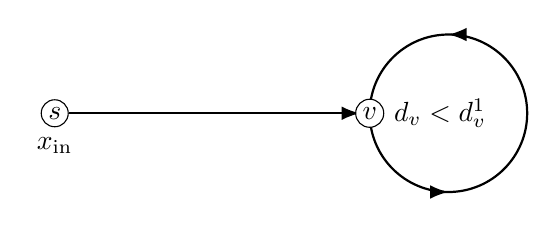
\begin{tikzpicture}[>=Latex,
  dot/.style={circle,draw,fill=white,inner sep=1.2pt},
  looparrow/.style={thick,postaction={decorate},
    decoration={markings,
      mark=at position 0.25 with {\arrow{Latex}},
      mark=at position 0.75 with {\arrow{Latex}}}}]
\node[dot,label=below:{$\xin$}] (s) at (0,0) {$s$};
\node  (v) at (4,0) {};
\draw[thick,-{Latex}] (s) -- (v);
\draw[looparrow] (5,0) circle [radius=1cm];
\node[dot, label=right:{$d_v < d^1_v$}]  at (v) {$v$};
\end{tikzpicture}
\caption{Illustration of an arbitrage path saved in  \texttt{save\_path}.}\label{fig:arb_path}
\end{figure}



\subsection{Arbitrage search}

Next, we discuss how to find the optimal input amount $\xin$. We begin by running Algorithm~\ref{alg:MBF} with $p = 0$ and a small initial input, for example, $\xin = 0.001$. This typically yields multiple arbitrage cycles. For each identified cycle, we apply a black-box optimization method – the Golden Section Search (GSS) – to find the optimal $\xin$.

GSS is a derivative-free optimization technique for finding the maximum (or minimum) of a unimodal function over a bounded interval. It is particularly suitable when the function’s analytic form is unknown or too expensive to compute, but function evaluations are available. GSS progressively narrows the interval of interest using the golden ratio, requiring only function values at strategically chosen points. In our setting, we use GSS to identify the input amount $\xin$ that maximizes arbitrage profit along a given cycle.

 
\subsection{Optimizations}

To reduce computation time, we divide the graph into subgraphs and solve the problem independently for each subgraph. To compute the subgraphs, we remove the start node $s$ and identify the resulting connected components. We then form each subgraph by reintroducing the start node $s$ and connecting it to a component. We execute the algorithm independently within each subgraph.

To further reduce runtime, we implemented the following memory management strategy.
\begin{itemize}[leftmargin=*, label=--]
    \item \textbf{Reference Counting:} By using \texttt{Rc<Vec<EdgeIndex>>}, the algorithm avoids deep cloning of cycle paths. This is especially beneficial when we detect many cycles.
    \item \textbf{Efficient Graph Updates:} We only update relevant subgraphs per block. This reduces recomputation.
    \item \textbf{BigUint Arithmetic:} We ensure that all calculations are safe from overflow. This is critical for financial computations.
\end{itemize}

\subsection{Summary:}
We have presented a Bellman-Ford algorithm with the following modifications:
\begin{itemize}
    \item We only consider cycles if they start and end at the designated start token (e.g., WETH).
    \item We use reference-counted vectors (\texttt{Rc<Vec<EdgeIndex>>}) to avoid unnecessary cloning.
    \item The algorithm skips cycles that revisit nodes, to avoid infinite loops.
    \item Profit calculation includes gas costs, and only exports cycles with net positive profit.
    \item The Golden Section Search adapts the input range if invalid points are encountered.
\end{itemize}


\bibliographystyle{splncs04}
\bibliography{references}

\end{document} 